\documentclass[11pt,a4paper]{article}
\usepackage[T1]{fontenc}
\usepackage[utf8]{inputenc}
\usepackage{libertinus}
\usepackage{microtype}
\usepackage[a4paper,margin=27mm,headheight=15pt]{geometry}
\usepackage{amsmath,amssymb,amsthm,mathtools,bm}
\usepackage{booktabs,array,longtable,enumitem}
\usepackage{xcolor,tcolorbox}
\tcbuselibrary{breakable}
\usepackage{fancyhdr,titlesec,needspace}
\usepackage{tikz}
\usetikzlibrary{arrows.meta}
\usepackage{hyperref}
\usepackage[nameinlink,noabbrev]{cleveref}
\definecolor{ink}{RGB}{29,54,77}
\definecolor{accent}{RGB}{35,89,105}
\hypersetup{colorlinks=true,linkcolor=ink,citecolor=accent,urlcolor=accent,
 pdftitle={The Endpoint Geometry of Common-Digit Fabius Laws},
 pdfauthor={OpenAI ChatGPT},
 pdfsubject={Joint small deviations, copula tails, continuum constraints, and Gaussianization}}
\titleformat{\section}{\Large\bfseries\color{ink}}{\thesection}{.65em}{}
\titleformat{\subsection}{\large\bfseries\color{ink}}{\thesubsection}{.65em}{}
\pagestyle{fancy}\fancyhf{}
\fancyhead[L]{\small Common-digit Fabius laws}
\fancyhead[R]{\small Endpoint geometry}
\fancyfoot[C]{\thepage}
\renewcommand{\headrulewidth}{.35pt}
\newtheorem{theorem}{Theorem}[section]
\newtheorem{proposition}[theorem]{Proposition}
\newtheorem{lemma}[theorem]{Lemma}
\newtheorem{corollary}[theorem]{Corollary}
\theoremstyle{definition}
\newtheorem{definition}[theorem]{Definition}
\newtheorem{example}[theorem]{Example}
\newtheorem{question}[theorem]{Research question}
\theoremstyle{remark}
\newtheorem{remark}[theorem]{Remark}
\newcommand{\PP}{\mathbb P}
\newcommand{\EE}{\mathbb E}
\newcommand{\RR}{\mathbb R}
\newcommand{\NN}{\mathbb N}
\newcommand{\ind}{\mathbf 1}
\newcommand{\Var}{\operatorname{Var}}
\newcommand{\Corr}{\operatorname{Corr}}
\newcommand{\sech}{\operatorname{sech}}
\newcommand{\argmax}{\operatorname*{arg\,max}}
\newcommand{\supp}{\operatorname{supp}}
\newcommand{\dd}{\,\mathrm d}
\newcommand{\pos}[1]{\left(#1\right)_+}
\newcommand{\sumi}{\sum_{i=1}^d}
\newcommand{\repoSHA}{\texttt{e1afd75e35a4de734d5aa47aec5cdb917b82ed3e}}
\newtcolorbox{resultbox}[1]{breakable,colback=accent!4,colframe=accent!65,
 title=\textbf{#1},boxrule=.5pt,arc=1mm}
\setlist[enumerate]{leftmargin=2em,itemsep=.35em}
\setlist[itemize]{leftmargin=1.6em,itemsep=.25em}
\setlength{\emergencystretch}{2em}
\allowdisplaybreaks[2]
\numberwithin{equation}{section}

\begin{document}
\begin{titlepage}
\thispagestyle{empty}
\vspace*{13mm}
{\small\sffamily\color{accent} PROVEIT RESEARCH CONTRIBUTION\par}
\vspace{8mm}
{\Huge\bfseries\color{ink} The Endpoint Geometry\\[3mm]
of Common-Digit\\[3mm]Fabius Laws\par}
\vspace{9mm}
{\Large Sharp joint small deviations, copula universality,\\[2mm]
continuum sampling, and noncommuting Gaussian limits\par}
\vspace{13mm}
\begin{resultbox}{The central mechanism}
Shared digits do not force shared extremes. A joint lower-tail event charges
one cost for each digit, determined by the strongest active parameter
constraint. The resulting upper envelope yields an explicit quadratic rate,
a block-simplex correction, and exact residual tail-dependence exponents.
\end{resultbox}
\vspace{9mm}
{\large Prepared for Vladimir Reshetnikov\par}
\vspace{2mm}
{\large 29 September 2026\par}
\vfill
\noindent\begin{minipage}{\textwidth}
\small
\textbf{Status.} A research manuscript with complete written proofs and
reproducible finite checks. No Lean or Rocq formalization is claimed.
The novelty claim is limited to the contribution developed here relative to
the inspected repository report; absolute historical priority has not been
established.\par\medskip
\textbf{Repository snapshot.} \repoSHA\par
\textbf{Source area.} \texttt{Analysis/FabiusFunction}; common-digit
geometric-uniform laws and the report's open endpoint-dependence program.
\end{minipage}
\end{titlepage}

\begin{abstract}
Let $U_0,U_1,\ldots$ be independent uniform random variables and couple all
parameters through the same digits,
$X_q=(1-q)\sum_{n\ge0}q^nU_n$. At $q=1/2$ the marginal distribution
function is the Fabius function. The existing ProveIt common-digit report
determines support geometry and a Gaussianization limit, but leaves endpoint
dependence as a research direction. We derive a joint small-deviation theory
whose governing object is the upper envelope
$h_a(x)=\max(0,a_i-\lambda_i x:1\le i\le d)$, where
$q_i=e^{-\lambda_i}$. In a fixed nondegenerate envelope chamber,
\[
\log\PP(X_{q_i}\le e^{-a_i t}\ \forall i)
=-I(a)t^2-T(a)t\log t+A(a)t+O((\log t)^2),
\]
with all coefficients explicit. The proof uses independent simplex blocks
and small transition strips rather than an unproved saddle-point inversion.
For digits with density $c z^{\beta-1}(1+O(z^\delta))$ at zero, we obtain
the corresponding sharp expansion and show that marginal standardization
removes $c$, all weight normalizations, and even $\beta$ from the leading
copula rate. A log-digit log-concavity argument proves actual regular
variation along power rays, not merely a logarithmic equivalent.

For $A>B>0$ and uniform digits, the diagonal copula exponent is
$\kappa=2\sqrt A/(\sqrt A+\sqrt B)$; hence the Ledford--Tawn coefficient is
$\eta=(1+\sqrt{B/A})/2$. We calculate the first stretched-exponential
correction, the complete bivariate phase diagram, and a finite-dimensional
formula that becomes $1+\tfrac14\log(A/B)$ under a continuum of parameter
constraints. Equally spaced logarithms of the $\lambda_i$ uniquely maximize
the finite-sample exponent. Finally, common hyperbolic parameter translation
keeps Pearson correlation exactly constant and gives a Gaussian limit, yet
its Gaussian and extreme-tail limits do not commute. We give exact finite
probability certificates, reproducible checks, limitations, and a prioritized
research agenda.
\end{abstract}

\setcounter{tocdepth}{1}
\tableofcontents
\clearpage

\section{The question, the contribution, and its boundary}
\label{sec:scope}

\subsection{What is inherited and what is addressed}
The classical Fabius construction provides a compactly supported smooth
probability law through an infinite series of independent uniform random
variables \cite{Fabius,Arias}. The ProveIt report \emph{Common-Digit Fabius
Zonoids} \cite{RepoCommon} couples the geometric-uniform laws at distinct
parameters with the \emph{same} digit sequence. It develops their support
zonotopes, covariance geometry, cumulants, parameter jets, and a Gaussian
limit under hyperbolic translation. Its section on inverse-Fabius copula
endpoint laws proposes boundary transseries and conditional extreme-event
asymptotics.

This manuscript studies the missing \emph{probability mass near the common
lower corner}. Exact support boundaries alone do not determine that mass.
Two random variables can have a smooth joint density, very strong positive
correlation, and a highly constrained common support, while simultaneous
extreme quantiles are nevertheless asymptotically independent. We quantify
that phenomenon and explain its mechanism.

The inspected source is pinned to the repository snapshot on the title
page. Its explicit conjecture \texttt{conj:copula-endpoints} concerns
\emph{boundary curves} and their transseries. We do not claim to prove that
entire conjecture. Our theorems resolve the associated joint lower-tail
rate problem and its first correction; conditioning on a threshold event is
also covered. Conditioning on an exact coordinate value, complete boundary
transseries, and bounded periodic terms remain separate questions.

\subsection{A map of the results}
\begin{center}
\begin{tabular}{p{.26\textwidth}p{.61\textwidth}}
\toprule
Result & Content and scope\\
\midrule
Envelope law & Finite and compact-continuum joint lower-tail rates; a direct
independent-box proof.\\[2mm]
Sharp expansion & Explicit $t^2$, $t\log t$, and $t$ terms with
$O((\log t)^2)$ remainder in fixed strict chambers.\\[2mm]
Copula universality & Endpoint-index-independent leading exponent and an
explicit $\sqrt{\log(1/u)}$ correction.\\[2mm]
Regular variation & Genuine power-ray regular variation when the
log-digit density is log-concave, including uniform and beta-power digits.\\[2mm]
Parameter sampling & Closed formulas for any finite diagonal, its continuum
limit, and optimal finite placement.\\[2mm]
Gaussian comparison & Constant-correlation Gaussianization does not commute
with extreme-quantile asymptotics.\\
\bottomrule
\end{tabular}
\end{center}

The elementary simplex integral, Pr\'ekopa's marginal theorem, regular
variation terminology, and the classical Gaussian tail calculation are not
new. They are identified where used. The proposed contribution is the
explicit envelope/simplex theory and its consequences for this common-digit
family. A focused literature search did not establish an earlier identical
result, but that is not a certification of historical priority.

\subsection{Conventions and the interpretation of errors}
All logarithms are natural. Parameters and dimension are fixed unless a
limit is explicitly stated. An $O$-constant may depend on those parameters
and on the digit law. Uniform error claims are made only on compact subsets
of a specified strict chamber. In particular, no uniformity as two distinct
parameters coalesce is implicit. Every asymptotic statement is a written
mathematical theorem of this manuscript; the accompanying program checks
finite identities and certificates, not infinite limiting assertions.

\section{The model and the geometry of an upper envelope}
\label{sec:geometry}

Let $V_0,V_1,\ldots$ be independent identically distributed random variables
in $[0,1]$. Set
\begin{equation}
 q_i=e^{-\lambda_i},\qquad w_i=1-e^{-\lambda_i},\qquad
 X_i=w_i\sum_{n=0}^{\infty}e^{-\lambda_i n}V_n,
 \qquad \lambda_i>0.
 \label{eq:model}
\end{equation}
The series converges absolutely and $0\le X_i\le1$. The uniform case is
$V_n=U_n\sim\operatorname{Unif}[0,1]$. We assume the $\lambda_i$ are
distinct; repeated coordinates can be consolidated by retaining the most
restrictive threshold.

For $a=(a_1,\ldots,a_d)\in(0,\infty)^d$ define
\begin{align}
 E_t(a)&=\{X_i\le e^{-a_i t}:1\le i\le d\},\label{eq:event}\\
 h_a(x)&=\max\{0,a_1-\lambda_1x,\ldots,a_d-\lambda_dx\},\label{eq:envelope}\\
 I(a)&=\int_0^\infty h_a(x)\dd x,
 &T(a)&=\max_i\frac{a_i}{\lambda_i}.
 \label{eq:rate}
\end{align}
For each $i$, let $\ell_i(a)$ be the length of the interval on which the
$i$th line is the unique positive maximizer. Empty intervals have length
zero. Ties occur at finitely many abscissae and do not affect lengths.
The positive envelope occupies $[0,T(a))$.

\begin{definition}[Strict envelope chamber]
A parameter vector $a$ lies in a strict chamber when the list of active
lines is unchanged by sufficiently small perturbations of $a$, all active
intervals have positive length, the active line at $x=0$ is unique, and no
inactive line touches a positive envelope vertex or the terminal vertex.
Equivalently, the relevant intersection and dominance inequalities are
strict. A one-line envelope with all other lines strictly inactive is
included.
\end{definition}

\begin{lemma}[Envelope calculus]
\label{lem:envelope}
The function $I$ is convex, continuously differentiable on
$(0,\infty)^d$, positively homogeneous of degree two, and quadratic on each
strict chamber. Moreover,
\begin{equation}
 \partial_{a_i}I(a)=\ell_i(a),\qquad
 \sum_i\ell_i=T,
 \qquad \sum_i\lambda_i\ell_i=\max_i a_i,
 \qquad \sum_i a_i\ell_i=2I(a).
 \label{eq:envelope-identities}
\end{equation}
If the active list, from left to right, is $i_1,\ldots,i_m$, then
$\lambda_{i_1}>\cdots>\lambda_{i_m}$ and
\begin{equation}
 I(a)=\frac{a_{i_m}^2}{2\lambda_{i_m}}
 +\sum_{j=1}^{m-1}
 \frac{(a_{i_j}-a_{i_{j+1}})^2}
 {2(\lambda_{i_j}-\lambda_{i_{j+1}})}.
 \label{eq:active-formula}
\end{equation}
\end{lemma}
\begin{proof}
Convexity follows by integrating a maximum of affine functions of $a$.
The substitution $x=cy$ gives $I(ca)=c^2I(a)$ for $c>0$.
Distinct slopes imply that the maximizer is unique away from finitely many
points. On a compact neighborhood of $a$, every positive envelope is
supported in a common bounded interval. Dominated convergence applied to
difference quotients therefore gives $\partial_{a_i}I=\ell_i$.
The same argument applied to the maximizing indicators proves continuity
of these derivatives, including at chamber walls.

The active intervals partition $[0,T]$, proving the first length identity.
Since $h'_a=-\lambda_i$ on the $i$th active interval, integrating $-h'_a$
gives $\sum\lambda_i\ell_i=h_a(0)=\max a_i$. Euler's identity for a
$C^1$ homogeneous function gives the final equality; alternatively integrate
$h_a-xh'_a$.

As $x$ increases, a line can replace the current maximum only if its slope
$-\lambda_i$ is larger. Consecutive active crossings occur at
\[
 x_j=\frac{a_{i_j}-a_{i_{j+1}}}{\lambda_{i_j}-\lambda_{i_{j+1}}},
 \quad x_0=0,\quad x_m=\frac{a_{i_m}}{\lambda_{i_m}}.
\]
Integrating $a_{i_j}-\lambda_{i_j}x$ over $[x_{j-1},x_j]$ and
collecting the endpoint terms gives \eqref{eq:active-formula}.
\end{proof}

Formula \eqref{eq:active-formula} is to be used with the \emph{actual}
upper-envelope list. Summing the displayed crossing terms over an arbitrary
ordering of all constraints is generally wrong.

\begin{figure}[ht]
\centering
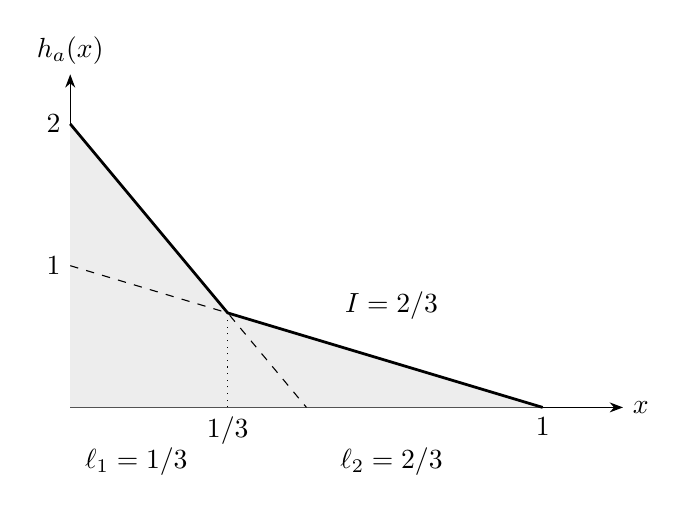
\begin{tikzpicture}[x=6cm,y=1.8cm,>=Stealth]
 \draw[->] (0,0)--(1.17,0) node[right] {$x$};
 \draw[->] (0,0)--(0,2.35) node[above] {$h_a(x)$};
 \fill[black!7] (0,0)--(0,2)--(0.333333,.666667)--(1,0)--cycle;
 \draw[dashed] (0,1)--(1,0);
 \draw[dashed] (0,2)--(.5,0);
 \draw[line width=1pt] (0,2)--(.333333,.666667)--(1,0);
 \draw[dotted] (.333333,0)--(.333333,.666667);
 \node[below] at (.333333,0) {$1/3$};
 \node[below] at (1,0) {$1$};
 \node[left] at (0,1) {$1$};\node[left] at (0,2) {$2$};
 \node at (.68,.72) {$I=2/3$};
 \node at (.14,-.38) {$\ell_1=1/3$};
 \node at (.68,-.38) {$\ell_2=2/3$};
\end{tikzpicture}
\caption{The envelope of $2-4x$, $1-x$, and zero. Early digits pay the
first constraint; later digits pay the second. The shaded area is the
leading rate.}
\label{fig:envelope}
\end{figure}

\section{The joint logarithmic law, including continuum constraints}
\label{sec:leading}

For this section only, assume the digit distribution function $F_V$
satisfies
\begin{equation}
 \frac{\log F_V(z)}{\log z}\longrightarrow\beta\in(0,\infty)
 \qquad(z\downarrow0).
 \label{eq:logendpoint}
\end{equation}
No density assumption is needed here.

\begin{theorem}[Upper-envelope small-deviation law]
\label{thm:leading}
Under \eqref{eq:logendpoint},
\begin{equation}
 \log\PP(E_t(a))=-\beta I(a)t^2+o(t^2).
 \label{eq:leading-law}
\end{equation}
If $\log F_V(z)=\beta\log z+O(1)$ uniformly for $0<z\le1$, the error
can be sharpened to $O(t\log t)$, locally uniformly in $a$.

The same statements hold with the finite set of constraints replaced by
all $\lambda\in[B,A]$, $0<B<A<\infty$, with continuous positive threshold
profile $a(\lambda)$ and $w(\lambda)=1-e^{-\lambda}$; replace the maximum
in \eqref{eq:envelope} by the supremum over this interval.
\end{theorem}
\begin{proof}
Write
\[
 b_{i,n}=a_it+\log w_i-\lambda_i n,
 \qquad b_n=\max_i b_{i,n}.
\]
If $E_t(a)$ occurs, positivity of every summand implies
$V_n\le\min(1,e^{-b_n})$ for each $n$. Independence gives the upper bound
\begin{equation}
 \PP(E_t(a))\le\prod_{n\ge0}F_V\bigl(e^{-\pos{b_n}}\bigr).
 \label{eq:box-upper}
\end{equation}
Only $O(t)$ factors differ from one. Since $\log w_i$ is bounded,
\begin{equation}
 \sum_{n\ge0}\pos{b_n}=t^2 I(a)+O(t).
 \label{eq:coarse-riemann}
\end{equation}
This is a Riemann sum for $t h_a(n/t)$; its support has length $O(t)$
and its normalized summand is uniformly Lipschitz.

For the converse, let $\lambda_{\min}=\min_i\lambda_i$ and choose
\[
 N=\left\lceil T(a)t+\frac{\log2}{\lambda_{\min}}\right\rceil.
\]
For every $i$ the normalized deterministic tail is bounded by
\[
 e^{a_it}w_i\sum_{n\ge N}e^{-\lambda_i n}
 =e^{a_it-\lambda_i N}\le\tfrac12.
\]
Impose the independent box conditions
\begin{equation}
 V_n\le c_n:=\min\left(1,\frac{e^{-b_n}}{2N}\right),
 \qquad 0\le n<N.
 \label{eq:box-lower}
\end{equation}
Each normalized core summand is at most $1/(2N)$, so these conditions
imply $E_t(a)$. Thus
\[
 \PP(E_t(a))\ge\prod_{n<N}F_V(c_n),\qquad
 \sum_{n<N}-\log c_n=t^2I(a)+O(t\log t).
\]
When $\log F_V(z)=\beta\log z+O(1)$, both product bounds give the
claimed quantitative error. Under the weaker condition
\eqref{eq:logendpoint}, for every $\varepsilon>0$ there is a constant
$C_\varepsilon$ such that, for all $s\ge0$,
\[
 |\log F_V(e^{-s})+\beta s|\le\varepsilon s+C_\varepsilon.
\]
Apply this to both products, divide by $t^2$, and then let
$\varepsilon\downarrow0$.

For the continuum case use
$b_n=\sup_{\lambda\in[B,A]}(a(\lambda)t+\log w(\lambda)-\lambda n)$.
The same deterministic implication, independence, and single common box
remain valid. Compactness bounds all supports, slopes, and normalization
constants. The resulting envelope is Lipschitz and decreasing until zero,
so the Riemann estimate and the uniform tail cutoff hold without change.
The event is measurable: the series defining $X_\lambda$ is uniformly
convergent on $[B,A]$, and continuous parameter constraints can be checked
on a fixed countable dense subset.
\end{proof}

\begin{remark}[Why the maximum, not the sum?]
Charging a separate independent cost for each parameter would produce
$\sum_i a_i^2/(2\lambda_i)$. That double-counts a digit which is already
small enough to satisfy several constraints. The correct leading cost is
one maximum per digit, and hence the area of one upper envelope. The
inequalities
\begin{equation}
 \max_i\frac{a_i^2}{2\lambda_i}\le I(a)
 \le\sum_i\frac{a_i^2}{2\lambda_i}
 \label{eq:rate-bounds}
\end{equation}
are immediate, but their usually strict gap contains the dependence
information.
\end{remark}

\section{A sharp three-scale expansion by independent simplex blocks}
\label{sec:sharp}

For the refined results assume that the digits have a density on $[0,1]$
with
\begin{equation}
 f(z)=c z^{\beta-1}\bigl(1+O(z^\delta)\bigr),
 \qquad c,\beta,\delta>0,
 \qquad z\downarrow0.
 \label{eq:density}
\end{equation}
This includes uniform digits ($\beta=c=1$) and
$\operatorname{Beta}(\beta,1)$ digits ($c=\beta$).

\begin{theorem}[Sharp joint lower-tail expansion]
\label{thm:sharp}
Suppose \eqref{eq:density} holds and $a$ is in a strict envelope chamber.
Then, as $t\to\infty$,
\begin{equation}
 \log\PP(E_t(a))
 =-\beta I(a)t^2-\beta T(a)t\log t+A_{\beta,c}(a)t
 +O((\log t)^2),
 \label{eq:sharp-law}
\end{equation}
where
\begin{equation}
 \begin{split}
 A_{\beta,c}(a)={}&\beta T(a)-\frac{\beta}{2}\max_i a_i\\
 &-\beta\sum_{\ell_i>0}\ell_i\log(\beta w_i\ell_i)
 +T(a)\log\bigl(c\Gamma(\beta)\bigr).
 \end{split}
 \label{eq:A}
\end{equation}
The error is uniform on compact subsets of a strict chamber. For uniform
digits,
\begin{equation}
 A(a)=T(a)-\frac12\max_i a_i
       -\sum_{\ell_i>0}\ell_i\log(w_i\ell_i).
 \label{eq:A-uniform}
\end{equation}
\end{theorem}

The $t\log t$ term is an entropy cost for making a sum of order $t$
positive coordinates small. The active block lengths tell us how many
coordinates each constraint must control. The proof below also supplies
finite computable bounds; it does not assume a multivariate saddle-point
formula.

\subsection{The simplex calculation and the refined lattice sum}

\begin{lemma}[Weighted Dirichlet simplex]
\label{lem:simplex}
For $N\ge0$, positive $A_1,\ldots,A_N$, $b>0$, and $\beta>0$,
\begin{equation}
 \int_{\substack{u_j\ge0\\\sum_j A_ju_j\le b}}
       \prod_{j=1}^N c u_j^{\beta-1}\dd u_j
 =\frac{(c\Gamma(\beta))^N b^{\beta N}}
 {\Gamma(\beta N+1)\prod_{j=1}^N A_j^\beta}.
 \label{eq:simplex}
\end{equation}
When $b\le\min_j A_j$, this simplex lies in $[0,1]^N$.
\end{lemma}
\begin{proof}
Substitute $y_j=A_ju_j/b$. The remaining Dirichlet integral is
$\Gamma(\beta)^N/\Gamma(\beta N+1)$, obtained by iterating the beta
integral, or by introducing the slack coordinate
$y_{N+1}=1-\sum_{j=1}^N y_j$ with exponent zero. The assertion about the
cube follows from $u_j\le b/A_j$. The empty integral is one.
\end{proof}

\begin{lemma}[Lattice cost]
\label{lem:lattice}
Let $b_{i,n}=a_it+\log w_i-\lambda_i n$ and
$b_n=\max_i b_{i,n}$. In a fixed strict chamber,
\begin{equation}
 S(t):=\sum_{n\ge0}\pos{b_n}
 =I(a)t^2+\frac12\max_i a_i\,t
    +t\sum_i\ell_i(a)\log w_i+O(1).
 \label{eq:lattice}
\end{equation}
If $N_i$ counts indices assigned to active line $i$, with only
$O(\log t)$ indices near the crossings or the final zero omitted, then
$N_i=t\ell_i+O(\log t)$ and
\begin{equation}
 \begin{split}
 \sum_i\log\Gamma(\beta N_i+1)
 ={}&\beta Tt\log t
  +\beta t\sum_{\ell_i>0}\ell_i\log(\beta\ell_i)
  -\beta Tt+O((\log t)^2).
 \end{split}
 \label{eq:factorial}
\end{equation}
\end{lemma}
\begin{proof}
The sum of a piecewise linear compactly supported function on a unit grid
is its integral plus half its value at zero, with an error bounded by a
constant times the sum of its finitely many slope jumps. One elementary
proof uses the trapezoidal rule: it is exact on every grid cell not
containing a breakpoint, and the error on a cell containing a breakpoint is
bounded by its slope jump. Apply this to
$x\mapsto t h_a(x/t)$, whose slopes are fixed. Thus
\[
 \sum_{n\ge0}t h_a(n/t)=I(a)t^2+\tfrac12 h_a(0)t+O(1).
\]
Adding the fixed intercept shifts $\log w_i$ moves each crossing by
$O(1)$ indices. Away from those finitely many indices it adds exactly
$\log w_i$ on the $i$th active block. The affected indices have bounded
\emph{differences} between competing lines; their correction is $O(1)$.
This proves \eqref{eq:lattice}.

The index counts follow from the interval lengths. Stirling's formula gives
\[
 \log\Gamma(\beta N+1)=\beta N\log(\beta N)-\beta N+O(\log(N+2)).
\]
Changing $N=t\ell_i$ by $O(\log t)$ changes the right side by
$O((\log t)^2)$ when $\ell_i>0$. Summing over the fixed active list proves
\eqref{eq:factorial}. Strict-chamber compactness bounds the nonzero lengths
away from zero and the crossing slopes away from degeneracy.
\end{proof}

\subsection{The upper bound}
Fix a constant $K>2$ sufficiently large that $K\delta>2$. Retain all
indices with $b_n\ge K\log t$, and assign each to its maximizing line.
Let $B_i^+$ be the resulting block and $N_i^+=|B_i^+|$. The necessary
conditions
\[
 \sum_{n\in B_i^+}e^{b_{i,n}}V_n\le1
\]
use disjoint digits. Within each necessary simplex every coordinate is at
most $t^{-K}$. Consequently \eqref{eq:density} can be used uniformly:
replacing the joint density there by $\prod c v_n^{\beta-1}$ changes the
logarithm of its integral by $O(t^{1-K\delta})$. Extending the integration
to the full nonnegative simplex is an upper bound, and
\cref{lem:simplex} gives
\begin{equation}
 \begin{split}
 \log\PP(E_t(a))\le{}&-\beta\sum_{i}\sum_{n\in B_i^+}b_{i,n}
 +\sum_iN_i^+\log(c\Gamma(\beta))\\
 &-\sum_i\log\Gamma(\beta N_i^++1)+O(1).
 \end{split}
 \label{eq:sharp-upper}
\end{equation}
Only $O(\log t)$ positive indices near the terminal zero are omitted,
and their total cost is $O((\log t)^2)$. In particular the double sum in
\eqref{eq:sharp-upper} is $S(t)+O((\log t)^2)$. Substituting
\cref{lem:lattice} proves the upper half of \eqref{eq:sharp-law}.

\subsection{A matching lower bound and why transition strips matter}
Set
\[
 \varepsilon=t^{-K},\qquad
 N=\left\lceil\max_i\frac{a_it+K\log t}{\lambda_i}\right\rceil.
\]
All normalized deterministic tails are at most $\varepsilon$. An index
$n<N$ belongs to core $B_i$ when
\begin{equation}
 b_{i,n}\ge K\log t,\qquad
 b_{i,n}-b_{j,n}\ge K\log t\quad(j\ne i).
 \label{eq:cores}
\end{equation}
Let $S$ be the residual set. In a strict chamber there are only
$M=|S|=O(\log t)$ residual indices: they lie in logarithmic-width strips
around the finitely many crossings and around the final zero. Each active
core has $|B_i|=t\ell_i+O(\log t)$.

On every core impose the simplex constraint
\[
 \sum_{n\in B_i}e^{b_{i,n}}V_n\le b_t,
 \qquad b_t=1-(d+2)\varepsilon,
\]
and on residual indices impose
\begin{equation}
 V_n\le\min\left(1,\frac{e^{-b_n}\varepsilon}{\max(1,M)}\right).
 \label{eq:strip-caps}
\end{equation}
For coordinate $i$, its own core contributes at most $b_t$, every other
core contributes at most $\varepsilon b_t$, all residual indices together
contribute at most $\varepsilon$, and the tail contributes at most
$\varepsilon$. Thus the total is less than one for all large $t$.
Inactive coordinates have no own core and satisfy an even smaller bound.
The constructed event is therefore contained in $E_t(a)$.

The core simplexes lie in $[0,t^{-K}]^{|B_i|}$, so the density estimate and
\cref{lem:simplex} give their probabilities with a bounded logarithmic
error. The budget factor contributes
$\beta\sum_i|B_i|\log b_t=O(t^{1-K})$. For residual indices,
\eqref{eq:density} implies the global comparison
$\log F_V(z)=\beta\log z+O(1)$ on $(0,1]$. Hence their log probability is
\[
 -\beta\sum_{n\in S}\pos{b_n}+O((\log t)^2).
\]
The extra $K\log t+\log\max(1,M)$ cost per strip index is responsible
for the stated remainder. Combining cores and strips restores
$-\beta S(t)$, up to $O((\log t)^2)$. The total numbers of active core
indices differ from $t\ell_i$ by only $O(\log t)$, so
\eqref{eq:factorial} applies. This proves the matching lower bound and
completes \cref{thm:sharp}.

\begin{remark}[A potentially serious proof error avoided]
A strip near an \emph{interior} crossing can contain $O(\log t)$ indices
each with cost $\Theta(t)$. Its total base cost is not
$O((\log t)^2)$. It would be wrong to discard those digits. The lower
bound above pays their original $\beta b_n$ costs explicitly and loses
only the extra logarithmic safety factors. That is what makes the linear
coefficient in \eqref{eq:sharp-law} valid.
\end{remark}

\begin{corollary}[Scalar specialization]
\label{cor:scalar}
For one parameter $\lambda$, $w=1-e^{-\lambda}$, and $s\to\infty$,
\begin{equation}
 \begin{split}
 -\log\PP(X\le e^{-s})
 ={}&\frac{\beta s^2}{2\lambda}
     +\frac{\beta s}{\lambda}\log s-D_{\lambda,\beta,c}s
     +O((\log s)^2),\\
 D_{\lambda,\beta,c}
 ={}&\frac{\beta}{\lambda}-\frac{\beta}{2}
 -\frac{\beta}{\lambda}\log\frac{\beta w}{\lambda}
 +\frac1\lambda\log(c\Gamma(\beta)).
 \end{split}
 \label{eq:scalar}
\end{equation}
\end{corollary}
This scalar order of expansion is a consistency check and an input to
marginal standardization, not a claim to supersede the repository's much
finer one-parameter Fabius asymptotics. The $n=0$ indexing and the factor
$w=1-e^{-\lambda}$ both matter for the linear coefficient.

\section{Marginal standardization and universal copula asymptotics}
\label{sec:copula}

Write $F_i$ for the marginal distribution function of $X_i$ and $Q_i$ for
its inverse near zero. Under \eqref{eq:density}, $F_i$ is continuous and
strictly increasing sufficiently close to zero. Indeed, a sufficiently
small positive tail has positive probability, and the first digit has a
strictly positive density near zero; conditioning on that tail gives
positive mass to each small open interval. The first digit also makes the
law atomless. Thus the inverses used below are unambiguous for small
arguments.

Define the lower copula by
\begin{equation}
 C(u_1,\ldots,u_d)=\PP(X_i\le Q_i(u_i):1\le i\le d).
 \label{eq:copula}
\end{equation}
For a power-ray vector $\alpha\in(0,\infty)^d$ put
\begin{equation}
 b_i=\sqrt{2\lambda_i\alpha_i},\quad
 K(\alpha)=I(b),\quad
 H(\alpha)=\sum_{\ell_i(b)>0}\ell_i(b)
     \log\frac{b_i/\lambda_i}{\ell_i(b)}.
 \label{eq:KH}
\end{equation}
The envelope and lengths here use the \emph{canonical} intercepts $b_i$,
without $\beta$.

\begin{theorem}[Universal copula rate and first correction]
\label{thm:copula}
Assume \eqref{eq:density}. For every positive $\alpha$,
\begin{equation}
 \lim_{L\to\infty}
 \frac{\log C(e^{-\alpha_1L},\ldots,e^{-\alpha_dL})}{L}
 =-K(\alpha).
 \label{eq:copula-leading}
\end{equation}
If $b$ lies in a strict envelope chamber, then
\begin{equation}
 \log C(e^{-\alpha_1L},\ldots,e^{-\alpha_dL})
 =-K(\alpha)L+\sqrt{\beta L}\,H(\alpha)
       +O((\log L)^2).
 \label{eq:copula-sharp}
\end{equation}
In particular, the leading rate is independent of $c$ and $\beta$;
$H$ is independent of $c$ and the weight factors $w_i$. Moreover,
\begin{equation}
 \max_i\alpha_i\le K(\alpha)\le\sum_i\alpha_i,
 \qquad H(\alpha)\ge0.
 \label{eq:copula-bounds}
\end{equation}
In a strict chamber $H=0$ exactly when a single line is active.
\end{theorem}

\subsection{Quantile inversion with the needed accuracy}
Let $t=\sqrt L$ and $\widetilde b_i=b_i/\sqrt\beta$. Then
\begin{equation}
 -\log Q_i(e^{-\alpha_iL})
 =\widetilde b_i t-\log t+d_i
      +O((\log t)^2/t),
 \label{eq:quantile}
\end{equation}
where
\begin{equation}
 d_i=1-\log\frac{w_i\beta\widetilde b_i}{\lambda_i}
   +\frac1\beta\log(c\Gamma(\beta))-\frac{\lambda_i}{2}.
 \label{eq:quantile-d}
\end{equation}
To verify this, substitute $s=\widetilde b_i t-\log t+d$ into
\eqref{eq:scalar}. The quadratic term gives $\alpha_i t^2$ and a
$-(\beta\widetilde b_i/\lambda_i)t\log t$ contribution. The
$s\log s$ term cancels the latter. The remaining coefficient of $t$
vanishes precisely for \eqref{eq:quantile-d}; the residual is
$O((\log t)^2)$. This substitution is also a rigorous inversion: changing
$s$ by $\pm M(\log t)^2/t$ changes the explicit main expression by
$\pm(\beta\widetilde b_i/\lambda_i)M(\log t)^2+o((\log t)^2)$.
Choose $M$ larger than the uniform error constant and use monotonicity to
bracket the true inverse. No differentiated remainder is assumed.

\subsection{The cancellation which produces universality}
Set
\[
 a_i(t)=\widetilde b_i+\frac{-\log t+d_i}{t}
                    +O((\log t)^2/t^2).
\]
For a strict chamber these vectors remain in one compact chamber
neighborhood. Applying \cref{thm:sharp} uniformly gives
\[
 -\beta I(a(t))t^2-\beta T(a(t))t\log t+A_{\beta,c}(a(t))t
 +O((\log t)^2).
\]
By \cref{lem:envelope} and piecewise quadraticity,
\[
 I(a(t))=I(\widetilde b)+\frac1t
 \sum_i\ell_i(\widetilde b)(-\log t+d_i)
 +O((\log t)^2/t^2).
\]
All $t\log t$ terms cancel because $\sum\ell_i=T$. The coefficient of
$t$ is
\[
 A_{\beta,c}(\widetilde b)-\beta\sum_i\ell_i(\widetilde b)d_i.
\]
Insert \eqref{eq:A} and \eqref{eq:quantile-d}. The terms containing
$\log(c\Gamma(\beta))$, $\log w_i$, and the free term $\beta T$
cancel. The remaining endpoint terms cancel by
$\sum_i\lambda_i\ell_i(\widetilde b)=\max_i\widetilde b_i$. What remains is
\[
 \beta\sum_i\ell_i(\widetilde b)
      \log\frac{\widetilde b_i/\lambda_i}{\ell_i(\widetilde b)}
 =\sqrt\beta\,H(\alpha).
\]
Homogeneity gives $\beta I(\widetilde b)=I(b)=K(\alpha)$, proving
\eqref{eq:copula-sharp}.

For the leading formula at a chamber wall, the scalar leading equivalent
in \cref{cor:scalar} still gives
$-\log Q_i(e^{-\alpha_iL})/\sqrt L\to\widetilde b_i$.
Use the locally uniform bound of \cref{thm:leading} and continuity of $I$.
The bounds for $K$ follow from \eqref{eq:rate-bounds}. An active interval
for line $i$ lies in $[0,b_i/\lambda_i]$, so
$\ell_i\le b_i/\lambda_i$ and every summand in $H$ is nonnegative.
With two or more active lines, at least one such inclusion is strict; with
only one it is an equality. This finishes the proof.

\begin{remark}[Endpoint universality has a precise meaning]
Universality here is invariance under replacing the uniform digit law by a
law satisfying \eqref{eq:density}, \emph{after its own marginals are
standardized}. It does not assert that the unstandardized probabilities,
whole copulas, covariances, or lower-order bounded oscillations coincide.
The endpoint exponent $\beta$ survives at the square-root scale.
\end{remark}

\section{From logarithmic rates to genuine regular variation}
\label{sec:RV}

An expansion with an $O((\log L)^2)$ remainder does \emph{not} by itself
imply regular variation: that remainder could oscillate too fast under a
fixed increment of $L$. To justify the standard residual-dependence
terminology, a separate argument is required. We give one using convexity.

Assume in this section that \eqref{eq:density} holds and the density
\begin{equation}
 g(z)=e^{-z}f(e^{-z})\ind_{\{z\ge0\}}
 \label{eq:logdigit}
\end{equation}
of $Z=-\log V$ is log-concave on $\RR$. Both uniform and
$\operatorname{Beta}(\beta,1)$ digits satisfy this hypothesis, since
$g(z)=\beta e^{-\beta z}\ind_{\{z\ge0\}}$ in the latter case.

\begin{lemma}[Convexity in log-threshold coordinates]
\label{lem:convexG}
The function
\begin{equation}
 G(s)=-\log\PP(X_i\le e^{-s_i}:1\le i\le d)
 \label{eq:G}
\end{equation}
is finite, convex, and coordinatewise nondecreasing on $\RR^d$.
\end{lemma}
\begin{proof}
For the first $N$ digits, the feasible set in $(s,z)$ is
\[
 z_n\ge0,\qquad
 \sum_{n<N}\exp(s_i+\log w_i-\lambda_i n-z_n)\le1
 \quad(1\le i\le d).
\]
It is convex, as each displayed exponential sum is convex. Its indicator
is log-concave in the extended sense. Multiplying by the log-concave
product density $\prod_{n<N}g(z_n)$ preserves log-concavity.
Pr\'ekopa's marginal theorem \cite{Prekopa} therefore makes the finite
probability log-concave in $s$. These probabilities decrease to the
infinite-series probability; the defining log-concavity inequality passes
to the limit. The limit is strictly positive for every finite $s$ by the
box construction. Taking minus its logarithm proves convexity. Monotonicity
is immediate from the events.
\end{proof}

\begin{lemma}[Asymptotic slopes of a convex rate]
\label{lem:grad}
Let $s_t/t\to a\in(0,\infty)^d$ and let $p_t$ be any subgradient of
$G$ at $s_t$. Then
\begin{equation}
 \frac{p_t}{t}\longrightarrow\beta\nabla I(a)
 =\beta(\ell_1(a),\ldots,\ell_d(a)).
 \label{eq:gradient-limit}
\end{equation}
\end{lemma}
\begin{proof}
By the box estimate, $G(tx)=\beta t^2I(x)+O(t\log t)$ uniformly for
$x$ in any compact subset of the positive orthant. Apply the subgradient
inequality at $s_t$ with increments $\pm\varepsilon t e_i$.
After division by $\varepsilon t^2$, it bounds $p_{t,i}/t$ between the
backward and forward difference quotients of $\beta I$ at $s_t/t$,
plus $O(\log t/(\varepsilon t))$. First let $t\to\infty$, then
$\varepsilon\downarrow0$, and use the continuous differentiability in
\cref{lem:envelope}. A finite convex function on $\RR^d$ has subgradients
at every point, so the argument applies to all choices.
\end{proof}

\begin{theorem}[Power-ray regular variation]
\label{thm:RV}
Under the assumptions of this section, for every $\alpha_i>0$ and $k>0$,
\begin{equation}
 \lim_{u\downarrow0}
 \frac{C((ku)^{\alpha_1},\ldots,(ku)^{\alpha_d})}
      {C(u^{\alpha_1},\ldots,u^{\alpha_d})}
 =k^{K(\alpha)}.
 \label{eq:RV}
\end{equation}
This includes chamber boundaries. Thus the copula restricted to any fixed
power ray is regularly varying at zero with index $K(\alpha)$.
\end{theorem}
\begin{proof}
Put $s_i(L)=-\log Q_i(e^{-\alpha_iL})$ and
$\widetilde b_i=\sqrt{2\lambda_i\alpha_i/\beta}$. Scalar leading
asymptotics give $s_i(L)\sim\widetilde b_i\sqrt L$. For a fixed real
$r$, the scalar version of \cref{lem:grad}, together with the two
subgradient bounds for an increment of a convex function, gives
\begin{equation}
 s_i(L+r)-s_i(L)=\frac{r\widetilde b_i}{2\sqrt L}+o(L^{-1/2}).
 \label{eq:quantile-increment}
\end{equation}
Here is the detail needed to avoid differentiating an asymptotic series.
The exact scalar identity is $G_i(s_i(L))=\alpha_iL$. Subgradients at
both endpoints are asymptotic to
$\beta\widetilde b_i\sqrt L/\lambda_i$. Their sandwich first bounds
the inverse increment by $O(L^{-1/2})$, and then evaluates it as
$\alpha_i r\lambda_i/(\beta\widetilde b_i\sqrt L)$, which is
\eqref{eq:quantile-increment}. Negative $r$ follows by reversing the
endpoints.

Apply the multivariate subgradient sandwich to $G$ at $s(L)$ and
$s(L+r)$. By \cref{lem:grad} the two subgradients, divided by $\sqrt L$,
converge to $\beta\ell(\widetilde b)$. Hence
\[
 G(s(L+r))-G(s(L))\longrightarrow
 \frac{r\beta}{2}\sum_i\widetilde b_i\ell_i(\widetilde b)
 =r\beta I(\widetilde b)=rK(\alpha).
\]
Take $r=-\log k$ and exponentiate the negative difference.
\end{proof}

In the weak lower-tail dependence notation of Tankov \cite{Tankov}, the
result gives
\begin{equation}
 \chi(\alpha)=\frac{\max_i\alpha_i}{K(\alpha)}.
 \label{eq:weak-function}
\end{equation}
For the diagonal in two dimensions, genuine regular variation yields the
Ledford--Tawn representation
$C(u,u)=u^{1/\eta}\mathcal L(u)$ with $\mathcal L$ slowly varying at
zero \cite{LedfordTawn}. Thus $\eta=1/K(1,1)$ is justified in the usual
sense, not merely defined by a logarithmic ratio.

\begin{remark}[What is not implied]
Power-ray regular variation is not a proof of a full multivariate hidden
regular-variation measure, angular limit, or copula-density asymptotic.
For general digits satisfying \eqref{eq:density} but not log-digit
log-concavity, \cref{thm:copula} still holds; \cref{thm:RV} is not
asserted without an additional argument.
\end{remark}

\section{The complete bivariate phase diagram}
\label{sec:bivariate}

Let the two decay rates be $A>B>0$, and let the corresponding raw
threshold intercepts be $a,b>0$. The envelope consists of zero,
$a-Ax$, and $b-Bx$.

\begin{proposition}[Three phases]
\label{prop:phases}
The raw rate is
\begin{equation}
 I(a,b)=
 \begin{cases}
 b^2/(2B),&a\le b,\\[1mm]
 b^2/(2B)+(a-b)^2/(2(A-B)),&b<a<(A/B)b,\\[1mm]
 a^2/(2A),&a\ge(A/B)b.
 \end{cases}
 \label{eq:phases}
\end{equation}
In the middle phase the active lengths are
\begin{equation}
 \ell_1=\frac{a-b}{A-B},\qquad
 \ell_2=\frac bB-\frac{a-b}{A-B}.
 \label{eq:two-lengths}
\end{equation}
For copula exponents $\alpha,\gamma>0$, put
$a=\sqrt{2A\alpha}$ and $b=\sqrt{2B\gamma}$. Then
\begin{equation}
 K(\alpha,\gamma)=
 \begin{cases}
 \gamma,&\alpha\le(B/A)\gamma,\\[1mm]
 \displaystyle\gamma+
 \frac{(\sqrt{A\alpha}-\sqrt{B\gamma})^2}{A-B},
 &(B/A)\gamma<\alpha<(A/B)\gamma,\\[2mm]
 \alpha,&\alpha\ge(A/B)\gamma.
 \end{cases}
 \label{eq:copula-phases}
\end{equation}
\end{proposition}
\begin{proof}
If $a\le b$, the slower line begins higher and decreases more slowly,
so it dominates. If $a/A\ge b/B$, the faster line remains higher until
the other line reaches zero. In the remaining case they switch at
$x_0=(a-b)/(A-B)$ before the slower line reaches zero. Integrate the
first line on $[0,x_0]$ and the second on $[x_0,b/B]$.
Substitution of the canonical intercepts gives \eqref{eq:copula-phases}.
\end{proof}

The leading function is $C^1$ across both boundaries, as the general
geometry predicts. Its second derivatives change there. In a one-line
phase, an additional parameter constraint is free \emph{at the leading
logarithmic scale}; this does not mean the corresponding event is exactly
redundant at finite thresholds.

\begin{theorem}[Diagonal exponent and explicit correction]
\label{thm:diagonal}
For uniform digits and $A>B>0$, put $L=\log(1/u)$. Then
\begin{equation}
 \log C(u,u)=-\kappa L+H\sqrt L+O((\log L)^2),
 \label{eq:diagonal-expansion}
\end{equation}
where
\begin{equation}
 \boxed{\quad
 \kappa=\frac{2\sqrt A}{\sqrt A+\sqrt B},\qquad
 H=\sqrt{\frac2B}\log\left(1+\sqrt{\frac BA}\right).
 \quad}
 \label{eq:diagonal-kH}
\end{equation}
The lower-tail dependence coefficient is zero, while the residual
coefficients are
\begin{equation}
 \lambda_L:=\lim_{u\downarrow0}\frac{C(u,u)}u=0,\qquad
 \eta=\frac{1+\sqrt{B/A}}2,\qquad
 \overline\chi=2\eta-1=\sqrt{B/A}.
 \label{eq:residual}
\end{equation}
For digits satisfying \eqref{eq:density}, the same logarithmic expansion
holds with $H$ replaced by $\sqrt\beta H$. The regular-variation
interpretation of $\eta$ additionally uses the assumption of
\cref{thm:RV}.
\end{theorem}
\begin{proof}
With $a=\sqrt{2A}$ and $b=\sqrt{2B}$, both lines are active and
\[
 \ell_1=\frac{\sqrt2}{\sqrt A+\sqrt B},\qquad
 \ell_2=\frac{\sqrt2\sqrt A}{\sqrt B(\sqrt A+\sqrt B)}.
\]
Formula \eqref{eq:copula-phases} gives $\kappa$. Both ratios
$(a/A)/\ell_1$ and $(b/B)/\ell_2$ equal $1+\sqrt{B/A}$.
Their length sum is $\sqrt{2/B}$, proving the displayed $H$.
Because $1<\kappa<2$, \eqref{eq:diagonal-expansion} implies
$C(u,u)/u\to0$. The residual formulas follow from \cref{thm:RV} and
the definitions in \cite{LedfordTawn,Tankov}.
\end{proof}

For uniform digits, replacing each digit by $1-U_n$ preserves the joint
law and replaces each $X_i$ by $1-X_i$. Therefore the same results hold
at the common upper corner. More generally, if a digit density has
endpoint powers $\beta_0$ at zero and $\beta_1$ at one, apply the lower
corner theorem separately to $V$ and $1-V$. The leading standardized
exponent is the same, but the square-root corrections use
$\sqrt{\beta_0}$ and $\sqrt{\beta_1}$ respectively.

\subsection{An explicit Fabius example}
Take
\[
 q=\frac12,\qquad r=2^{-1/4},\qquad
 A=\log2,\quad B=\frac14\log2.
\]
The first marginal CDF is the Fabius function. Here
\begin{equation}
 \kappa=\frac43,\quad \eta=\frac34,\quad
 \overline\chi=\frac12,\quad
 H=\sqrt{\frac8{\log2}}\log\frac32
   =1.377481422290\ldots.
 \label{eq:fabius-example}
\end{equation}
Consequently the conditional extreme-threshold probability is
\begin{equation}
 \begin{split}
 &\PP\bigl(F_r(X_r)\le u\mid F_q(X_q)\le u\bigr)\\
 &\hspace{10mm}=
 u^{1/3}\exp\left\{H\sqrt{\log(1/u)}
       +O\bigl((\log\log(1/u))^2\bigr)\right\}.
 \end{split}
 \label{eq:conditional-threshold}
\end{equation}
This tends to zero despite the complete sharing of the underlying digits.
The conditioning event is an inequality of probability $u$, not the
zero-probability equality $X_q=x$.

\subsection{A nonuniform coalescence warning}
As $A\downarrow B$, the fixed-parameter exponent tends to one, consistent
with identical coordinates. But the displayed fixed-chamber correction
tends to $\sqrt{2/B}\log2$, whereas at exact equality $C(u,u)=u$ has no
such term. There is no contradiction: the proof removes strips whose
width constants involve inverse slope gaps. Those constants diverge as
$A-B\to0$, and fixed-chamber asymptotics are not uniform in this limit.
A simultaneous coalescence/extreme-value transition is a genuine further
problem, not resolved by substituting $A=B$ into \eqref{eq:diagonal-kH}.

\section{Many parameters, a continuum, and optimal placement}
\label{sec:continuum}

\begin{theorem}[Finite diagonal exponent]
\label{thm:finite-d}
Order the parameters as
$\lambda_1>\lambda_2>\cdots>\lambda_d>0$. For uniform digits, and also
for every digit density satisfying \eqref{eq:density},
\begin{equation}
 \lim_{u\downarrow0}
 \frac{\log C(u,\ldots,u)}{\log u}
 =\kappa_d
 =1+\sum_{j=1}^{d-1}
 \frac{\sqrt{\lambda_j}-\sqrt{\lambda_{j+1}}}
      {\sqrt{\lambda_j}+\sqrt{\lambda_{j+1}}}.
 \label{eq:kappa-d}
\end{equation}
All canonical lines are active, so the sharp correction in
\cref{thm:copula} also applies.
\end{theorem}
\begin{proof}
The intercepts are $\sqrt{2\lambda_i}$. Consecutive crossings are
\[
 x_j=\frac{\sqrt2}{\sqrt{\lambda_j}+\sqrt{\lambda_{j+1}}},
 \quad x_0=0,\quad x_d=\sqrt{2/\lambda_d}.
\]
These abscissae are strictly increasing. More explicitly, the graph of
$\sqrt{2\lambda}$ is strictly concave in $\lambda$, so intermediate
nodes lie strictly above chords connecting nonadjacent nodes. Hence
successive intersections indeed describe the upper envelope; no line is
skipped. Apply \eqref{eq:active-formula}. The last-line triangle has area
one, and each crossing term simplifies to the displayed adjacent ratio.
\end{proof}

\begin{definition}[Continuum diagonal probability]
For fixed $0<B<A$, let
\begin{equation}
 \mathcal C_{[B,A]}(u)=
 \PP\left(F_{e^{-\lambda}}(X_{e^{-\lambda}})\le u
                     \text{ for every }\lambda\in[B,A]\right).
 \label{eq:continuum-C}
\end{equation}
This is the probability of a common extreme-quantile event along the
entire parameter curve, not a finite-dimensional copula with an informal
infinite index.
\end{definition}

\begin{theorem}[Continuum exponent]
\label{thm:continuum}
For digits satisfying \eqref{eq:density},
\begin{equation}
 \boxed{\qquad
 \lim_{u\downarrow0}
 \frac{\log\mathcal C_{[B,A]}(u)}{\log u}
 =\kappa_\infty=1+\frac14\log\frac AB.
 \qquad}
 \label{eq:kappa-infty}
\end{equation}
For uniform digits the logarithm equals
$-\kappa_\infty L+O(\sqrt L\log L)$, where $L=\log(1/u)$.
No continuum analogue of the sharper $H\sqrt L$ term is asserted here.
\end{theorem}
\begin{proof}
The series $X_{e^{-\lambda}}$ converges uniformly and continuously in
$\lambda\in[B,A]$. Its marginal CDFs are jointly continuous by coupling
and atomlessness. The positive density near zero gives continuous inverse
CDFs for sufficiently small arguments, uniformly on compact parameter
intervals. The event in \eqref{eq:continuum-C} can therefore be checked on
a countable dense set.

The scalar box bounds, uniformly for $\lambda\in[B,A]$, imply
\[
 -\log Q_{e^{-\lambda}}(e^{-L})
 =\sqrt{2\lambda L/\beta}+O(\log L).
\]
This weaker uniform inversion follows already from
$-\log F_{e^{-\lambda}}(e^{-s})=\beta s^2/(2\lambda)+O(s\log s)$;
no interchange of finite-dimensional sharp limits is involved. Apply the
continuum version of \cref{thm:leading}. Homogeneity cancels $\beta$,
and the relevant canonical envelope is
\begin{equation}
 h(x)=\sup_{\lambda\in[B,A]}\pos{\sqrt{2\lambda}-\lambda x}
 =\begin{cases}
 \sqrt{2A}-Ax,&0\le x\le(2A)^{-1/2},\\
 (2x)^{-1},&(2A)^{-1/2}\le x\le(2B)^{-1/2},\\
 \sqrt{2B}-Bx,&(2B)^{-1/2}\le x\le\sqrt{2/B},\\
 0,&x\ge\sqrt{2/B}.
 \end{cases}
 \label{eq:continuum-envelope}
\end{equation}
Indeed, the unconstrained maximizer satisfies
$\lambda=1/(2x^2)$. The first and last linear pieces have areas $3/4$
and $1/4$; the middle piece has area $\tfrac14\log(A/B)$.
This proves the limit. The uniform box error and the $O(\log L)$
quantile error both contribute at most $O(\sqrt L\log L)$ to the
logarithm, proving the stated quantitative bound.
\end{proof}

\begin{theorem}[Optimal finite placement and saturation]
\label{thm:design}
Fix endpoints $\lambda_1=A$, $\lambda_d=B$ and $d\ge2$. Among distinct
ordered internal parameters, $\kappa_d$ is uniquely maximized by
\begin{equation}
 \lambda_j=A\exp\left(-\frac{j-1}{d-1}\log\frac AB\right),
 \qquad 1\le j\le d.
 \label{eq:optimal-mesh}
\end{equation}
Writing $D=\log(A/B)$, the optimum and its saturation gap are
\begin{align}
 \kappa_d^{\max}&=1+(d-1)\tanh\frac{D}{4(d-1)},\label{eq:kappa-opt}\\
 \kappa_\infty-\kappa_d^{\max}
 &=\frac{D^3}{192(d-1)^2}+O((d-1)^{-4}).\label{eq:gap}
\end{align}
Inserting any genuinely new parameter between two existing parameters
strictly increases the exponent.
\end{theorem}
\begin{proof}
Set $\Delta_j=\log\lambda_j-\log\lambda_{j+1}>0$. Then
$\sum\Delta_j=D$ and each adjacent term in \eqref{eq:kappa-d} is
$\tanh(\Delta_j/4)$. The function $\tanh x$ is strictly concave on
$(0,\infty)$, so Jensen's inequality gives
\eqref{eq:kappa-opt}, with equality precisely for all $\Delta_j$ equal.
Expand $\tanh x=x-x^3/3+O(x^5)$ to obtain \eqref{eq:gap}.
Finally, for $r,s>0$,
$\tanh(r+s)=(\tanh r+\tanh s)/(1+\tanh r\tanh s)
<\tanh r+\tanh s$; splitting a gap therefore increases the exponent.
\end{proof}

\begin{center}
\begin{tabular}{r r r r}
\toprule
$d$ & $\kappa_d^{\max}$ & $\kappa_\infty$ & $(d-1)^2(\kappa_\infty-\kappa_d^{\max})$\\
\midrule
2 & 1.600000000 & 1.693147181 & 0.093147181\\
3 & 1.666666667 & 1.693147181 & 0.105922056\\
5 & 1.686291501 & 1.693147181 & 0.109690873\\
9 & 1.691417870 & 1.693147181 & 0.110675888\\
17 & 1.692713880 & 1.693147181 & 0.110924946\\
33 & 1.693038794 & 1.693147181 & 0.110987388\\
\bottomrule
\end{tabular}

\end{center}
The table uses $A/B=16$. Its last column converges to
$(\log16)^3/192=0.111008\ldots$. The design criterion is specifically
maximization of the simultaneous extreme-quantile exponent. It is not a
claim of universal optimality for estimation, interpolation, or ordinary
mean-square prediction.

\Needspace{9\baselineskip}
\section{Why a Gaussian limit gets these extremes wrong}
\label{sec:gaussian}

\subsection{Pearson correlation and the true residual coefficient}
For any nondegenerate iid digit law with finite variance, the covariance
sum in \eqref{eq:model} gives
\begin{equation}
 \rho(q,r)=\Corr(X_q,X_r)
 =\frac{\sqrt{(1-q^2)(1-r^2)}}{1-qr}.
 \label{eq:rho}
\end{equation}
This calculation also appears in the common-digit source
\cite{RepoCommon}. For $q=e^{-A}$ and $r=e^{-B}$,
\begin{equation}
 \rho(q,r)=\frac{\sqrt{\sinh A\sinh B}}{\sinh((A+B)/2)}.
 \label{eq:rho-hyperbolic}
\end{equation}

\begin{proposition}[Correlation overstates Gaussian residual dependence]
\label{prop:rho}
For $A>B>0$,
\begin{equation}
 \rho(q,r)>\frac{2\sqrt{AB}}{A+B}>\sqrt{B/A}
 =\overline\chi_{\mathrm{common\ digit}}.
 \label{eq:rho-inequality}
\end{equation}
A Gaussian copula with correlation $\rho(q,r)$ has the smaller diagonal
exponent $2/(1+\rho(q,r))$, and therefore larger joint lower-tail
probabilities at the leading exponent scale than the common-digit copula.
\end{proposition}
\begin{proof}
The function $f(x)=\log(\sinh x/x)$ is strictly convex on $(0,\infty)$,
since
\[
 f''(x)=\frac1{x^2}-\frac1{\sinh^2x}>0.
\]
Its strict midpoint inequality inserted into
\eqref{eq:rho-hyperbolic} yields the first inequality. The second follows
from $2A/(A+B)>1$.

For completeness, if two standard normal variables have correlation
$\rho\in(0,1)$, their joint lower tail at $-z$ has logarithm
$-z^2/(1+\rho)+O(\log z)$. The upper bound follows by applying a
normal tail bound to their sum; a lower bound follows by integrating the
joint density over the square $[-z-z^{-1},-z]^2$. Since
$\log\Phi(-z)=-z^2/2+O(\log z)$, their copula exponent is
$2/(1+\rho)$, in agreement with the general Gaussian calculation in
\cite{Tankov}. Compare this with \eqref{eq:diagonal-kH}.
\end{proof}

\subsection{Fixed correlation, a Gaussian limit, and two different answers}
Let $v_2>v_1$ and $\delta=v_2-v_1>0$. For sufficiently large $T$ set
\begin{equation}
 q_1(T)=\tanh(T+v_1),\qquad q_2(T)=\tanh(T+v_2).
 \label{eq:translate}
\end{equation}
Denote their common-digit copula by $C_T$.

\begin{theorem}[Gaussian and extreme-tail limits do not commute]
\label{thm:noncommute}
For uniform digits the correlation in \eqref{eq:translate} is exactly
$\rho=\sech\delta$, independently of $T$, and $C_T$ converges pointwise
on $(0,1)^2$ to the Gaussian copula $C_\rho^{\mathrm G}$. Nevertheless,
\begin{align}
 \lim_{T\to\infty}\lim_{u\downarrow0}
 \frac{\log C_T(u,u)}{\log u}
 &=\frac2{1+e^{-\delta}},\label{eq:first-limit}\\
 \lim_{u\downarrow0}\lim_{T\to\infty}
 \frac{\log C_T(u,u)}{\log u}
 &=\frac2{1+\sech\delta}.
 \label{eq:second-limit}
\end{align}
The first value is strictly larger than the second.
\end{theorem}
\begin{proof}
The elementary hyperbolic subtraction formula transforms \eqref{eq:rho}
into $\sech(v_2-v_1)$, proving the exact correlation assertion.
The Gaussianization itself is present in \cite{RepoCommon}; we give a
short independent proof of precisely the finite-dimensional consequence
needed here.

The centered standardized variable is
\[
 Y_q=\sqrt{12(1-q^2)}\sum_{n\ge0}q^n(U_n-\tfrac12).
\]
For any fixed real coefficients $c_1,c_2$, the summands of
$c_1Y_{q_1(T)}+c_2Y_{q_2(T)}$ are independent, centered, and bounded in
absolute value by a deterministic number tending to zero. Their variance
sum is the constant
$c_1^2+c_2^2+2\rho c_1c_2$. The sum of their third absolute moments is
at most their maximum absolute bound times that variance sum, and hence
tends to zero. Taylor expansion of the characteristic functions, or the
Lindeberg argument, proves a centered normal limit with that variance.
Cram\'er--Wold gives the bivariate normal limit. Since the limiting
marginal CDFs are continuous and strictly increasing, the marginal
quantiles converge at each fixed $u\in(0,1)$; the joint convergence then
implies $C_T(u,v)\to C_\rho^{\mathrm G}(u,v)$.

For each fixed $T$, write $\lambda_i(T)=-\log q_i(T)$. The exact
common-digit exponent is
\[
 \kappa_T=\frac2{1+\sqrt{\lambda_2(T)/\lambda_1(T)}}.
\]
Since $-\log\tanh x\sim2e^{-2x}$,
$\sqrt{\lambda_2(T)/\lambda_1(T)}\to e^{-\delta}$.
This proves \eqref{eq:first-limit}. Taking $T\to\infty$ first gives
the Gaussian copula, whose exponent was calculated in the preceding
proof; this is \eqref{eq:second-limit}. Finally
$\sech\delta>e^{-\delta}$ for $\delta>0$.
\end{proof}

\begin{example}[A numerical separation with exact constants]
If $\delta=\log2$, Pearson correlation is $\sech(\log2)=4/5$ for
\emph{every} $T$. The extreme-tail-first limit is $4/3$, whereas the
Gaussian-first limit is $10/9$. Covariance does not merely converge to the
wrong predictor of endpoint behavior: it is unchanged throughout the
entire transition.
\end{example}

The distinction is structural. Gaussianization describes bounded
standardized fluctuations when the largest digit weight vanishes.
An endpoint event constrains an increasing number of positive digits
simultaneously. Its logarithmic cost depends on which geometric decay rate
is active at each digit index, information not determined by covariance.

\section{Finite probability certificates and reproducible checks}
\label{sec:certificates}

The preceding asymptotic proof has a finite, independently checkable core.
This is useful both for testing coefficients and for a future formalization.
The following certificate does not require equal-rate thresholds or any
asymptotic regime.

\begin{proposition}[Finite block certificate]
\label{prop:certificate}
Fix thresholds $x_i>0$ and an integer $N\ge1$, and put
\[
 A_{i,n}=\frac{w_iq_i^n}{x_i}\quad(0\le n<N),\qquad
 \tau_i=\frac{q_i^N}{x_i}.
\]
Partition $\{0,\ldots,N-1\}$ into disjoint cores $B_1,\ldots,B_d$
and a residual set $S$. Choose positive core budgets $b_j$ and caps
$0<c_n\le1$ for $n\in S$. For a nonempty core define
$R_{ij}=\max_{n\in B_j}A_{i,n}/A_{j,n}$, and set $R_{ij}=0$ for an
empty core. Suppose
\begin{align}
 b_j&\le\min_{n\in B_j}A_{j,n}\quad(B_j\ne\varnothing),
 \label{eq:certificate-cube}\\
 \sum_jR_{ij}b_j+\sum_{n\in S}A_{i,n}c_n+\tau_i&\le1
 \quad(1\le i\le d).
 \label{eq:certificate-budget}
\end{align}
For $\operatorname{Beta}(\beta,1)$ digits,
\begin{equation}
 \PP(X_i\le x_i\ \forall i)\ge
 \prod_j\frac{\Gamma(\beta+1)^{|B_j|}b_j^{\beta|B_j|}}
 {\Gamma(\beta|B_j|+1)\prod_{n\in B_j}A_{j,n}^\beta}
 \prod_{n\in S}c_n^\beta.
 \label{eq:certificate-lower}
\end{equation}
For any disjoint assigned blocks $D_j$ of finitely many digit indices,
an upper bound is
\begin{equation}
 \PP(X_i\le x_i\ \forall i)\le
 \prod_j\min\left(1,
 \frac{\Gamma(\beta+1)^{|D_j|}}
 {\Gamma(\beta|D_j|+1)\prod_{n\in D_j}A_{j,n}^\beta}\right).
 \label{eq:certificate-upper}
\end{equation}
For uniform digits, rational inputs make all quantities in these
certificates rational.
\end{proposition}
\begin{proof}
On core $B_j$ impose $\sum_{n\in B_j}A_{j,n}V_n\le b_j$ and on
$S$ impose $V_n\le c_n$. The row inequality
\eqref{eq:certificate-budget} proves that the whole normalized sum in
each coordinate is at most one, including its bounded infinite tail.
The cube condition lets \cref{lem:simplex} evaluate each core probability
exactly, and independence multiplies the disjoint factors. For the upper
bound, the full event implies
$\sum_{n\in D_j}A_{j,n}V_n\le1$ for each assigned block. Extend the
integration from the cube to the positive orthant, apply the same simplex
formula, and use independence. Intersecting with the trivial probability
bound one only improves the result.
\end{proof}

\subsection{What the included program actually checks}
The standard-library program \texttt{verify.py} performs 804 exact
rational envelope tests: randomized active-list identities, the full
bivariate phase formula on a rational grid, and finite diagonal formulas.
Its random seed is fixed. It also constructs an exact rational lower and
upper probability certificate for
\[
 (q_1,q_2)=(1/2,3/4),\qquad (x_1,x_2)=(2^{-20},2^{-15}).
\]
The certificate has $N=46$, core sizes $(4,4)$, and 38 residual digits.
Every row budget and cube inclusion is checked with Python
\texttt{Fraction} arithmetic; no floating-point sign decision is used
for those assertions. Decimal evaluations of the resulting exact bounds
are
\[
 -392.442411713\ldots\ \le\
 \log\PP(X_1\le2^{-20},X_2\le2^{-15})
 \ \le\ -231.988498892\ldots.
\]
These are deliberately simple certificates, not tight probability
estimates. Their decimal representations are ordinary floating-point
evaluations, not outward-rounded interval endpoints.

A separate numerical calculation checks the second-order copula
cancellation for 100 choices of $\beta,c$. It also generates the following
asymptotic table for uniform digits with
\[
 (\lambda_1,\lambda_2)=(4,1),\qquad (a_1,a_2)=(2,1).
\]
Here $I=2/3$, $T=1$, $\ell=(1/3,2/3)$, and
$A(a)=0.948459414\ldots$. The lower and upper columns show
\[
 \frac{\log(\text{certificate bound})+I t^2+Tt\log t}{t}.
\]
\begin{center}
\begin{tabular}{r r r r}
\toprule
$t$ & Lower certificate & $A(a)$ & Upper certificate\\
\midrule
100 & -1.125052 & 0.948459 & 0.889717\\
500 & 0.276169 & 0.948459 & 0.933357\\
2,000 & 0.708024 & 0.948459 & 0.943991\\
10,000 & 0.882048 & 0.948459 & 0.947413\\
50,000 & 0.930301 & 0.948459 & 0.948216\\
\bottomrule
\end{tabular}

\end{center}
Both certificates approach the predicted coefficient. The coefficient
itself need not lie between the two finite-$t$ entries, because the
normalized probability has its own nonzero remainder. Unlike the
rational certificate, this large-$t$ table is evaluated using ordinary
floating-point logarithms and gamma functions. It illustrates a proved
asymptotic mechanism; it is not an interval-certified experiment.

\subsection{Reproduction and trust boundary}
Run \texttt{python3 verify.py} in the package directory. It regenerates
\texttt{verification.txt}, the CSV table, the exact certificate metadata,
and the two LaTeX tables under \texttt{generated/}. Then run
\texttt{pdflatex article.tex} twice to rebuild this PDF. Only the Python
standard library is required for the checks. A standard TeX installation
with Libertinus, TikZ, and the listed document packages is required for
the PDF.

The exact checks verify finite arithmetic statements selected by the
program. Python itself is not a proof-assistant kernel, and no claim is
made that the program certifies the measure-theoretic passage to an
infinite series, Pr\'ekopa's theorem, or the asymptotic errors. Those are
proved in the text. Conversely, no plot or numerical trend is used as a
hypothesis in those proofs.

\section{Further research questions and a formalization roadmap}
\label{sec:questions}

The following problems are not claimed solved. They are ordered roughly
from a close extension of the present methods to a substantially broader
program.

\begin{question}[Bounded terms and joint periodic phases]
Can \eqref{eq:sharp-law} be continued through the $(\log t)^2$,
$\log t$, constant, and bounded oscillatory scales? The geometric lattice
suggests several phases, including the crossing indices and the terminal
cutoff. Determine when a genuine periodic or quasiperiodic function occurs,
and distinguish lattice effects from the errors introduced by the strip
construction. A multidimensional Laplace inversion would need a proved
uniform remainder, not just a formal saddle expansion.
\end{question}

\begin{question}[Conditioning on an exact coordinate]
Determine asymptotics of the joint density, conditional density, and
$\PP(X_r\le y\mid X_q=x)$ in a specified endpoint scaling. This would
approach the conditional-event problem suggested by the source report
more directly than \eqref{eq:conditional-threshold}. Differentiating the
current probability expansion is not justified and cannot be used as a
shortcut.
\end{question}

\begin{question}[Coalescing parameters]
Find a uniform transition law when $A-B\downarrow0$ simultaneously with
$u\downarrow0$. The mismatch of the fixed-chamber correction at exact
coalescence shows that a new scaling analysis is necessary. Identify the
correct crossover variable rather than assuming that fixed-parameter
asymptotics remain uniform.
\end{question}

\begin{question}[A simultaneous Gaussian/extreme limit]
In \cref{thm:noncommute}, let $L=\log(1/u)$ grow together with $T$.
Which regimes interpolate between $2/(1+\sech\delta)$ and
$2/(1+e^{-\delta})$? Because an individual largest standardized weight is
of order $e^{-T}$, the quantity $e^{-T}\sqrt L$ is a natural candidate
for locating a transition, but this is a heuristic scale, not a theorem.
A uniform moderate-deviation analysis could test and refine it.
\end{question}

\begin{question}[A continuum second-order law]
Compute the first correction to \eqref{eq:kappa-infty}. The middle
branch of \eqref{eq:continuum-envelope} is curved and has continuously
varying active parameters, so there is no fixed finite set of simplex
blocks. It is not legitimate to send $d\to\infty$ in the finite $H$
formula without controlling the growth of its error. Determine whether a
$\sqrt L\log L$ term survives and how it depends on the endpoint digit
index.
\end{question}

\begin{question}[Growing dimension and near-optimal meshes]
How fast may $d=d(L)$ grow while the finite-dimensional sharp expansion
remains uniform? Combine the gap in \eqref{eq:gap} with a uniform bound
on transition-strip losses. The rate formula gives a deterministic design
criterion; a growing-dimensional probability theorem would quantify when
that criterion predicts actual finite-threshold performance.
\end{question}

\begin{question}[Regular variation without log-digit log-concavity]
Does \cref{thm:RV} hold for every density satisfying
\eqref{eq:density}? The explicit logarithmic expansion alone is
insufficient. One possible route is a local ratio theorem for the core
simplexes which controls probability changes under $O(L^{-1/2})$
log-threshold increments and treats all transition strips uniformly.
\end{question}

\begin{question}[Hidden regular variation and angular laws]
Construct, when it exists, a full hidden limit measure beyond the power-ray
limits. Identify its natural scaling and angular component, and relate
changes of active envelope to changes in the limiting conditional digit
profile. The piecewise-quadratic $K$ provides a candidate rate geometry,
not the measure itself.
\end{question}

\begin{question}[Dependent digits]
Extend the envelope law to stationary Markov or mixing digits whose
small-value probabilities have controlled conditional powers. Determine
whether the leading cost is still an integral of a scalar envelope or
becomes a matrix or entropy-rate variational problem. The present proof
uses independence essentially in both its box and simplex steps.
\end{question}

\begin{question}[Signed sums and genuine parameter jets]
Parameter derivatives of $X_q$ introduce signed polynomial-geometric
coefficients. The one-digit necessary bounds used here then fail because
of cancellation. Develop a replacement for joint lower-corner events or
small norm balls of actual jets. Results for a positive scalar
polynomial-geometric series do not automatically solve this signed
multivariate problem.
\end{question}

\begin{question}[Distinguishing covariance from endpoint structure]
Can the exact relation $\overline\chi=\sqrt{B/A}$ be used to identify
relative geometric decay rates from extremes, and how does that compare
with covariance-based identification? Develop estimators and quantify
bias caused by the explicit $H\sqrt L$ correction. The latter can be
large at practical thresholds even when the limiting exponent is simple.
\end{question}

\subsection{A staged Lean/Rocq route}
The first useful formal target is \cref{prop:certificate}, not the entire
analytic manuscript. Encode rational weights, a partition of finite digit
indices, row budgets, and the simplex expression. A proved checker can
then turn an external proposed partition into a finite theorem, with a
transparent boundary between arithmetic verification and probability
semantics. The existing repository's emphasis on certificates makes this
a natural integration point.

A second stage formalizes finite upper envelopes: active-list correctness,
intersection ordering, area, and \eqref{eq:envelope-identities}. These
statements require only finite algebra and elementary integration. The
bivariate phase formulas and optimal-mesh inequalities can then be checked
independently of the full probability construction.

The analytic stages are more demanding: uniform convergence of the random
series, independent-box products, the Dirichlet simplex integral, the
transition-strip estimate, and local-uniform error bounds. Copula
standardization should follow only after a quantitative inverse-bracketing
lemma is available. The regular-variation route additionally needs a
suitable Pr\'ekopa theorem or a specialized proof for exponential digits.
This roadmap is a proposal; no unavailable library theorem or uncompiled
Lean code is presented as completed work.

\section{Conclusion}
The common-digit construction has two distinct geometries. Its central
fluctuations are governed by a covariance kernel and can become Gaussian.
Its simultaneous endpoint events are governed by an upper envelope of
geometric decay lines and by the volumes of independent simplex blocks.
The latter geometry yields explicit joint rates, first corrections,
residual coefficients, finite and continuum sampling formulas, and a
constant-correlation example of noncommuting Gaussian and extreme limits.

These are substantial answers to the endpoint-dependence program attached
to the repository's common-digit Fabius family. They do not replace the
remaining boundary-transseries, conditional-density, uniform-coalescence,
or formal-verification tasks. The package separates the proved statements,
classical inputs, finite computational checks, and unresolved questions so
that each next step has a precise mathematical target.

\appendix
\section{Source audit and reproducibility manifest}
\label{app:audit}

The mathematical baseline was the common-digit report at the pinned commit,
not an unpinned description of the repository. The repository root README,
Fabius README, and draft manifest were used to locate that report. Its
sections on the common-digit construction, copula support, Gaussianization,
and open endpoint laws were the relevant comparison points. The large
repository was not exhaustively audited, and no claim is made that every
historical draft or unpublished parallel contribution was inspected.

Targeted external checks covered the original Fabius construction,
Pr\'ekopa's marginal theorem, residual dependence, and weak copula tails.
They establish appropriate classical attribution, not exhaustive novelty.
The source report's scalar small-ball conjecture already has an editorial
correction in the inspected snapshot. We neither rely on its uncorrected
form nor describe the scalar specialization here as a new resolution of
that issue.

\begin{center}
\begin{tabular}{p{.35\textwidth}p{.51\textwidth}}
\toprule
Package item & Purpose\\
\midrule
\texttt{article.tex}, \texttt{article.pdf} & Complete manuscript and compiled
reading copy.\\[1mm]
\texttt{verify.py} & Exact finite checks, probability certificate, and
numerical tables; standard library only.\\[1mm]
\texttt{verification.txt} & Output of the included program from this build.\\[1mm]
\texttt{generated/} & Regenerated tables, CSV data, and exact-certificate
input/budget metadata.\\[1mm]
\texttt{README.md} & Build instructions and statement of proof status.\\[1mm]
\texttt{SOURCE\_AUDIT.md} & Pinned source locations, attribution, and novelty
limitations.\\
\bottomrule
\end{tabular}
\end{center}

\clearpage
\begin{thebibliography}{9}

\bibitem{RepoCommon}
Vladimir Reshetnikov, \emph{ProveIt}, repository research report
\emph{Common-Digit Fabius Zonoids: Exact volumes, hyperbolic-secant geometry,
Bernoulli Gaussianization, and parameter jets}, dated 30 August 2026,
with subsequent editorial notes. Snapshot \repoSHA.
{\raggedright Source path:
\path{Analysis/FabiusFunction/docs/semi-formalized-research-frontiers/drafts/representations/common_digit_fabius_zonoids_frontier_report/common_digit_fabius_zonoids.tex}.\par}
\href{https://github.com/VladimirReshetnikov/ProveIt/blob/e1afd75e35a4de734d5aa47aec5cdb917b82ed3e/Analysis/FabiusFunction/docs/semi-formalized-research-frontiers/drafts/representations/common_digit_fabius_zonoids_frontier_report/common_digit_fabius_zonoids.tex}{Pinned source on GitHub}.
The file identifies an AI-generated research-report author; the repository
owner is listed here for repository attribution, not as an inferred claim
of sole manuscript authorship.

\bibitem{Fabius}
J.~Fabius,
A probabilistic example of a nowhere analytic $C^\infty$-function,
\emph{Zeitschrift f\"ur Wahrscheinlichkeitstheorie und Verwandte Gebiete}
\textbf{5} (1966), 173--174.
\href{https://doi.org/10.1007/BF00536652}{doi:10.1007/BF00536652}.
A precursor report is retained by CWI:
\url{https://ir.cwi.nl/pub/8160}.

\bibitem{Arias}
J.~Arias de Reyna,
\emph{An infinitely differentiable function with compact support:
Definition and properties}, arXiv:1702.05442 (2017), English version of
an earlier Spanish article.
\url{https://arxiv.org/abs/1702.05442}.

\bibitem{Prekopa}
A.~Pr\'ekopa,
On logarithmic concave measures and functions,
\emph{Acta Scientiarum Mathematicarum (Szeged)} \textbf{34} (1973),
335--343. In particular, the marginalization theorem for log-concave
functions.
\url{https://acta.bibl.u-szeged.hu/14411/}.

\bibitem{LedfordTawn}
A.~W.~Ledford and J.~A.~Tawn,
Statistics for near independence in multivariate extreme values,
\emph{Biometrika} \textbf{83} (1996), no.~1, 169--187.
\href{https://doi.org/10.1093/biomet/83.1.169}{doi:10.1093/biomet/83.1.169}.

\bibitem{Tankov}
P.~Tankov,
Tails of weakly dependent random vectors,
\emph{Journal of Multivariate Analysis} \textbf{145} (2016), 73--86.
\href{https://doi.org/10.1016/j.jmva.2015.12.008}{doi:10.1016/j.jmva.2015.12.008}.
Preprint arXiv:1402.4683:
\url{https://arxiv.org/abs/1402.4683}.

\end{thebibliography}
\end{document}
